%%%%%%%% ICML 2025 EXAMPLE LATEX SUBMISSION FILE %%%%%%%%%%%%%%%%%

\documentclass{article}

% Recommended, but optional, packages for figures and better typesetting:
\usepackage{microtype}
\usepackage{graphicx}
\usepackage{subfigure}
\usepackage{booktabs} % for professional tables
\usepackage{amsmath}
\usepackage{bm}
\usepackage{multirow}

% hyperref makes hyperlinks in the resulting PDF.
% If your build breaks (sometimes temporarily if a hyperlink spans a page)
% please comment out the following usepackage line and replace
% \usepackage{icml2025} with \usepackage[nohyperref]{icml2025} above.
\usepackage{hyperref}


% Attempt to make hyperref and algorithmic work together better:
\newcommand{\theHalgorithm}{\arabic{algorithm}}

% Use the following line for the initial blind version submitted for review:
\usepackage{icml2025}

% If accepted, instead use the following line for the camera-ready submission:
% \usepackage[accepted]{icml2025}

% For theorems and such
\usepackage{amsmath}
\usepackage{amssymb}
\usepackage{mathtools}
\usepackage{amsthm}

% if you use cleveref..
\usepackage[capitalize,noabbrev]{cleveref}

%%%%%%%%%%%%%%%%%%%%%%%%%%%%%%%%
% THEOREMS
%%%%%%%%%%%%%%%%%%%%%%%%%%%%%%%%
\theoremstyle{plain}
\newtheorem{theorem}{Theorem}[section]
\newtheorem{proposition}[theorem]{Proposition}
\newtheorem{lemma}[theorem]{Lemma}
\newtheorem{corollary}[theorem]{Corollary}
\theoremstyle{definition}
\newtheorem{definition}[theorem]{Definition}
\newtheorem{assumption}[theorem]{Assumption}
\theoremstyle{remark}
\newtheorem{remark}[theorem]{Remark}

% Todonotes is useful during development; simply uncomment the next line
%    and comment out the line below the next line to turn off comments
%\usepackage[disable,textsize=tiny]{todonotes}
\usepackage[textsize=tiny]{todonotes}


% The \icmltitle you define below is probably too long as a header.
% Therefore, a short form for the running title is supplied here:
\icmltitlerunning{Submission for ICML 2025}

\begin{document}

\twocolumn[
\icmltitle{Thermal-SAM: Adversarial Prompt-Based Unsupervised Building Segmentation in Thermal Aerial Imagery – A Case Study in Turin}

% It is OKAY to include author information, even for blind
% submissions: the style file will automatically remove it for you
% unless you've provided the [accepted] option to the icml2025
% package.

% List of affiliations: The first argument should be a (short)
% identifier you will use later to specify author affiliations
% Academic affiliations should list Department, University, City, Region, Country
% Industry affiliations should list Company, City, Region, Country

% You can specify symbols, otherwise they are numbered in order.
% Ideally, you should not use this facility. Affiliations will be numbered
% in order of appearance and this is the preferred way.
\icmlsetsymbol{equal}{*}

\begin{icmlauthorlist}
\icmlauthor{Firstname1 Lastname1}{equal,yyy}
\icmlauthor{Firstname2 Lastname2}{equal,yyy,comp}
\icmlauthor{Firstname3 Lastname3}{comp}
\icmlauthor{Firstname4 Lastname4}{sch}
\icmlauthor{Firstname5 Lastname5}{yyy}
\icmlauthor{Firstname6 Lastname6}{sch,yyy,comp}
\icmlauthor{Firstname7 Lastname7}{comp}
%\icmlauthor{}{sch}
\icmlauthor{Firstname8 Lastname8}{sch}
\icmlauthor{Firstname8 Lastname8}{yyy,comp}
%\icmlauthor{}{sch}
%\icmlauthor{}{sch}
\end{icmlauthorlist}

\icmlaffiliation{yyy}{Department of XXX, University of YYY, Location, Country}
\icmlaffiliation{comp}{Company Name, Location, Country}
\icmlaffiliation{sch}{School of ZZZ, Institute of WWW, Location, Country}

\icmlcorrespondingauthor{Firstname1 Lastname1}{first1.last1@xxx.edu}
\icmlcorrespondingauthor{Firstname2 Lastname2}{first2.last2@www.uk}

% You may provide any keywords that you
% find helpful for describing your paper; these are used to populate
% the "keywords" metadata in the PDF but will not be shown in the document
\icmlkeywords{Machine Learning, ICML}

\vskip 0.3in
]

% this must go after the closing bracket ] following \twocolumn[ ...

% This command actually creates the footnote in the first column
% listing the affiliations and the copyright notice.
% The command takes one argument, which is text to display at the start of the footnote.
% The \icmlEqualContribution command is standard text for equal contribution.
% Remove it (just {}) if you do not need this facility.

%\printAffiliationsAndNotice{}  % leave blank if no need to mention equal contribution
% \printAffiliationsAndNotice{\icmlEqualContribution} % otherwise use the standard text.

\begin{abstract}
Thermal image building segmentation is essential for monitoring energy consumption and supporting environmental protection. Current segmentation methods are predominantly designed for RGB images, posing challenges for thermal images, especially when segmenting buildings of varied shapes from aerial views, due to their lower resolution, lack of detailed features, and channel differences. To address these challenges, we propose an unsupervised segmentation method Thermal-SAM, specifically for a new aerial thermal dataset from Turin, Italy. We enhance this method by incorporating color aerial images from the same region as an auxiliary modality to generate pseudo labels for unsupervised training. Our approach introduces an adversarial prompt-based pseudo-label generation method, utilizing several vision-language models, along with positive and negative prompts. Extensive experiments demonstrate that Thermal-SAM, surpasses state-of-the-art methods by more than 10\%.
\end{abstract}

\section{Introduction}
\label{introduction}


Global warming intensifies environmental challenges such as hurricanes and floods. Reducing energy consumption is crucial to mitigating these effects \cite{rogelj20132020}. Buildings account for 40\% of global energy use and emissions due to construction, heating, cooling, etc, \cite{nejat2015global}. Monitoring building temperatures with Unmanned Aerial Vehicle (UAV) infrared cameras is a promising approach to estimate energy use intensity (EUI) \cite{ham2013automated}. Thus, efficient building segmentation is vital. However, accurately segmenting buildings in UAV-captured thermal images is difficult since current segmentation methods are mainly designed for RGB images \cite{kirillov2023segment,chen2020blendmask}.

 

\begin{figure}[t]
\centering
\centerline{\includegraphics[scale=0.7 ]{figs/demo_image_offical.pdf}}
\caption{Images captured by aircraft in both spectrum.}
\label{demo}
\end{figure}

Visible cameras capture light in the RGB spectrum, providing detailed object information. In contrast, thermal images, captured by infrared cameras, consist of a single channel representing infrared intensity \cite{gade2014thermal}. Detailed visual data is crucial for object segmentation to classify objects and identify pixel-level edges, making RGB images more suitable for these tasks \cite{he2017mask,kirillov2023segment}. Figure~\ref{demo} shows the difference: buildings and cars are easily segmented in visible images, but difficult to discern in infrared images due to the lack of color information. The lower intensity of infrared radiation limits thermal image detail and resolution, posing challenges for accurate building segmentation and precise EUI prediction.

Current challenges for thermal image segmentation include a lack of thermal-based datasets and well-pretrained segmentation models. Most existing image segmentation datasets focus on RGB images from visible cameras \cite{zhou2017scene,lin2014microsoft}, leading to the development of powerful pretrained encoders for semantic and instance segmentation across various categories \cite{strudel2021segmenter,kirillov2023segment}. In contrast, thermal image segmentation mainly targets pedestrians \cite{wang2019thermal,altay2022use} and vehicles \cite{yang2015new,masouleh2019development}, as these are easier to annotate. Segmenting buildings in thermal images presents challenges, including low resolution, variable shapes, and unclear boundaries, resulting in a lack of annotated datasets and well-pretrained models.  Therefore, these challenges highlight the need for innovative, unsupervised segmentation methods tailored to this domain.

Based on this intuition, we propose Thermal-SAM, an unsupervised building thermal image segmentation model using a new constructed aerial thermal image dataset from Turin city. This model leverages adversarial prompts to enhance segmentation. This work focuses on \emph{Step 1}: extracting pixel-accurate thermal building footprints from mid-wave IR mosaics. Step 2—using those masks as inputs to predict building-level energy-use intensity (EUI)—is treated in a separate manuscript, currently under review. By isolating the segmentation stage here, we provide a stand-alone, reproducible baseline that downstream energy models can directly adopt.


\textbf{Contribution scope.}
This paper tackles \emph{Step 1} in a two-stage pipeline: extracting pixel-accurate thermal building footprints from mid-wave IR mosaics. Step 2—linking those masks to building-level EUI—is covered in a companion manuscript now under review. Downstream energy models can directly adopt the isolated segmentation results.
% Isolating the segmentation stage here provides a stand-alone, reproducible baseline that downstream energy models can directly adopt.

\textbf{Main contributions.}
\begin{itemize}
    \item \textbf{Thermal-SAM.} First unsupervised thermal-image model that segments buildings without human labels.
    \item \textbf{Vision–language synergy.} Hierarchical captioning supplies robust semantic cues for pseudo-labels.
    \item \textbf{Adversarial prompt generation.} A novel prompt scheme expands SAM’s capabilities to distorted IR imagery and boosts IoU by +10 pp over strong baselines.
\end{itemize}


\section{Related Works}

The field of unsupervised image segmentation has advanced significantly, addressing the challenges posed by reliance on human labeling. Notable methods include CutLER \cite{wang2023cut}, which introduces MaskCut, leveraging self-supervised learning with Vision Transformers \cite{dosovitskiy2020image} and DINO \cite{caron2021emerging} for class-agnostic object segmentation. Similarly, STEGO \cite{hamiltonunsupervised} employs clustering on DINO-extracted features for semantic segmentation, while U2Seg \cite{niu2024unsupervised} bridges semantic and instance segmentation using pseudo-labels from MaskCut, DINO, and clustering.  Despite these advancements, extending such unsupervised methods to building segmentation in thermal images remains largely unexplored and challenging. This is primarily due to the scarcity of high-quality, large-scale datasets of aerial-view thermal building images, as existing ones predominantly focus on pedestrians and vehicles \cite{liu2018real, li2020segmenting}.


\section{Methodology}



\begin{figure*}[t]
\centering
\centerline{
\includegraphics[scale=0.095 ]{figs/model_structure.pdf}}
\caption{Our unsupervised thermal image segmentation framework, Thermal-SAM, includes three modules: Zero-Shot Panoptic Segmentation, Adversarial Prompts-based Pseudo Label Generation, and Unsupervised Fine-tuning for Thermal Image Segmentation. }
\label{model}
\end{figure*}

\subsection{Overview}

As shown in Figure~\ref{model}, Thermal-SAM adopt SAM, OneFormer, CLIP-Seg, and Sentence Transformers to achieve robust unsupervised thermal building segmentation (descriptions are illustrated in Appendix A).



\subsection{Zero-Shot Panoptic Segmentation}

We first present our Thermal-SAM for panoptic segmentation of color imagery. Given an UAV image in visible view (color) $\bm{I}\in \mathbb{R}^{H\times W \times 3}$ and a paired infrared view (thermal) $\bm{T}\in \mathbb{R}^{H\times W}$, we map these two image by rotation $\mathcal{T}$  and shift $\bm{\Delta}$:
\begin{equation}
\bm{I}' = \mathcal{T}(\bm{I}) + \bm{\Delta}_{\bm{I}},
\label{eq1}
\end{equation}
where $\bm{I}'$ is the transformed color image. Subsequently, we crop and partition the color image and thermal image into smaller patches $\bm{P}^{(I)}_N$ and $\bm{P}^{(T)}_N$, respectively, where $N$ is number of patches, each of which retaining only valid regions unobscured by black pixels in the thermal image.

Next, we pass each visible view patch $\bm{P}^{(I)}_N$ into SAM, which outputs an instance mask and a set of segmented instance images:
\begin{equation}
\bm{M}^{(I)}_N; \bm{F}^{(I)} = \text{SAM}\Bigl(\bm{P}^{(I)}_N\Bigr),
\label{eq2}
\end{equation}
where $\bm{M}^{(I)}_N$ denotes the instance mask, and $\bm{F}^{(I)} = \{\bm{f}^{I}_1,..,\bm{f}^{I}_n\}$  represents the set of segmented instances extracted from  $\bm{P}^{(I)}_{i,j}$ (with $n$ being the total number of instances).

Then, for each segmented instance $\bm{f}^{I}_n$, we generate a coarse-grained image label $\bm{C}^{(I)(O)}_n$ using OneFormer and fine-grained image labels $\bm{C}^{(I)(B)}_n$ using BLIP2:
\begin{equation}
  \bm{C}^{(I)(B)}_n, \bm{C}^{(I)(O)}_n = \text{BLIP2}\bigl(\bm{f}^{I}_n\bigr), \text{OneFormer}\bigl(\bm{f}^{I}_n\bigr).
\label{eq3}
\end{equation}
The fine-grained labels include more details of the instance description. Finally,  we apply a Clip-Seg model to generate the final accurate labels:
\begin{equation}
\bm{C}^{(I)}_n = \operatorname{argmax}\bigl(\text{Clip-Seg}\bigl(\bm{f}^{I}_n, [\bm{C}^{(I)(O)}_n,\bm{C}^{(I)(B)}_n] \bigr)\bigl).
\label{eq4}
\end{equation}
The final step aggregates the labels of all instances in a patch:
\begin{equation}
\bm{C}^{(I)}_N = \{\bm{C}^{(I)}_1,..,\bm{C}^{(I)}_n\}.
\label{eq5}
\end{equation}
\subsection{Adversarial Prompts-based Pseudo Label Generation}
Given that Thermal-SAM is designed to segment all buildings from thermal images, we employ an adversarial prompts-based pseudo-label generation approach to select only building-related instances in the color aerial image.

We first compile a list of building-related words to serve as positive prompts $\bm{S}^+$ and a set of words that are semantically similar but do not actually refer to buildings as negative prompts $\bm{S}^-$. Then, we apply a Sentence Transformer to filter out building-irrelevant labels from the image labels $\bm{C}^{(I)}$ using cosine similarity $cos$: 
\begin{equation} 
\begin{aligned} 
\bm{Y}^{(I)}_N = &\{\bm{y}^{(I)}_k \mid \cos(\bm{C}^{(I)}_n, \bm{S}^+)
\geq \tau^+ \} \\
&\cap \{\bm{y}^{(I)}_k \mid \cos(\bm{C}^{(I)}_n, \bm{S}^+) < \tau^- \}, 
\end{aligned} 
\label{eq6} 
\end{equation}
where $\bm{Y}^{(I)}_N = \{\bm{y}^{(I)}_1,..,\bm{y}^{(I)}_k\}, \text{with} \ k<n$, $\tau^+$ is the threshold for selecting building-relevant labels, and $\tau^-$ is the threshold for filtering out building-irrelevant labels. 

Finally, we extract the building-related masks as segmentation labels for the next-step fine-tuning:
\begin{equation} 
\bm{M}^{(I)*}_N = \{ \bm{m}^{(I)}_k\mid \bm{y}^{(I)}_k \in \bm{Y}^{(I)}_N \} \ \text{and}\  \bm{m}^{(I)}_k \in \bm{M}^{(I)}_N.
\label{eq7} \end{equation}
\subsection{Unsupervised Fine-tuning for Thermal Image Segmentation}

The building-only mask by using Eq~\eqref{eq12}does not perfectly align with thermal images due to distortions between visible and infrared views. To address this, we use the masks $\bm{M}^{(I)*}_N$ as pseudo labels to fine‐tune SAM over a few epochs, enhancing SAM’s ability to segment thermal images without being compromised by the inaccuracies of the labels:
\begin{equation}
\bm{M}^{(T)*}_N = \operatorname{SAM}(\bm{M}^{(I)*}_N,\bm{P}^{(T)}_N; \theta), 
\label{eq8} \end{equation}
where $\theta$ is the tunable parameter. Finally, we manually select the best output between $\bm{M}^{(I)*}_N$ and $\bm{M}^{(T)*}_N$. Refer to Appendix A.1 for the detailed Thermal-SAM algorithm.
\begin{figure*}[htbp]
\centering
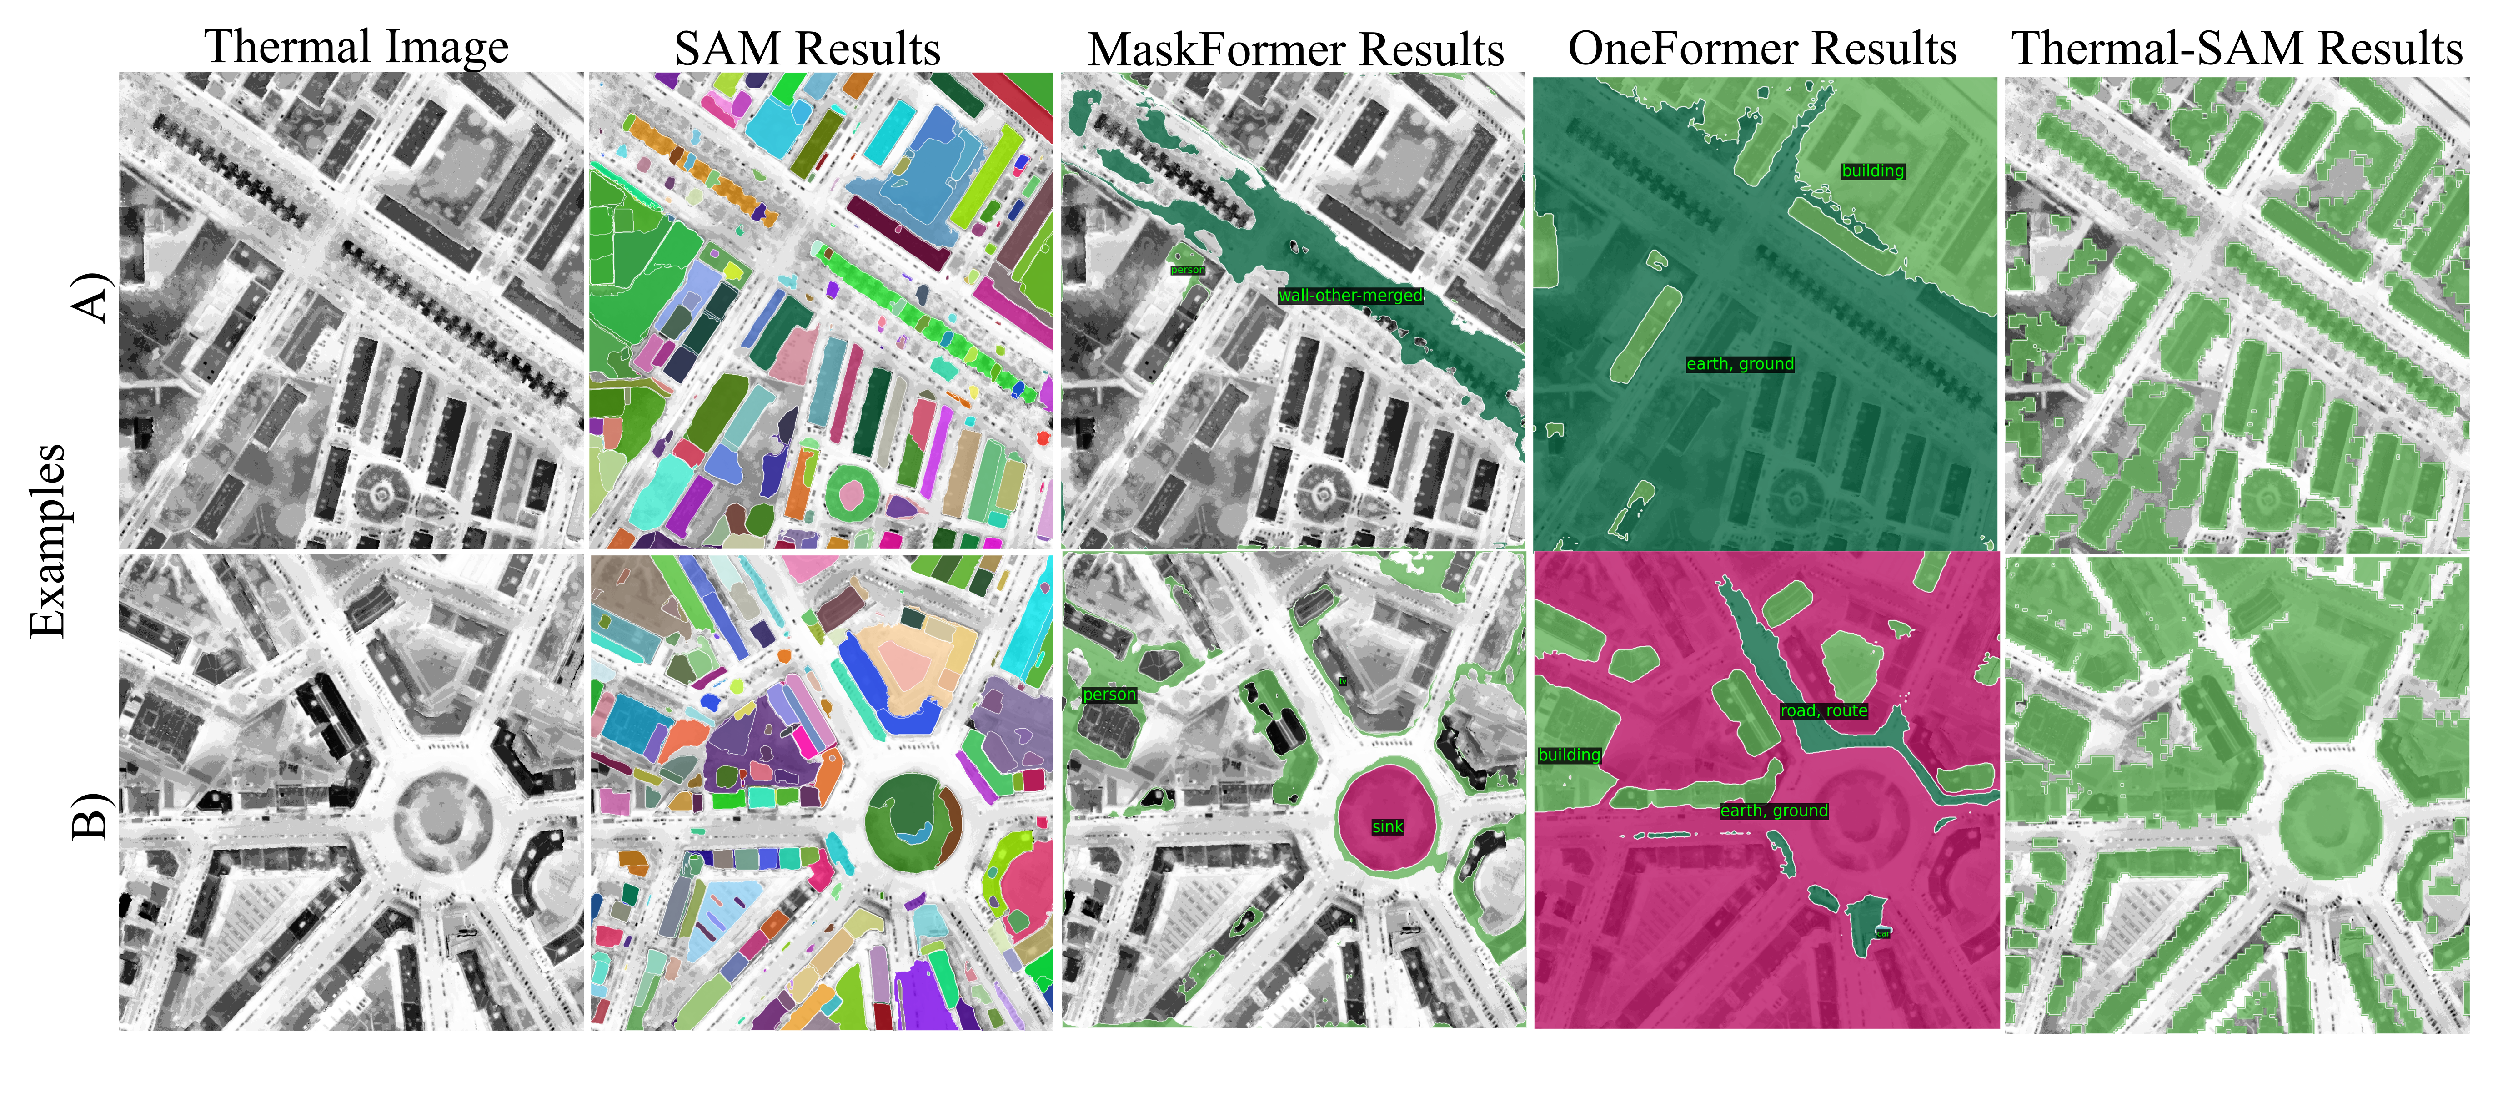
\includegraphics[height=0.4\linewidth]{figs/eval_baseline.pdf}
\caption{Qualitative Comparison of Building Segmentation: Thermal-SAM vs. Baseline Models}
\label{fig:segresults}
\end{figure*}
\section{Experiments}
\subsection{Dataset Description}
In this study, we captured aerial imagery of Turin, Italy, on March 23, 2023.  Thermal images were captured by FLIR A8581 MWIR HD camera, concurrently, color aerial images were captured from the same vantage (More description and data preprocessing please refer to Appendix A.2 and A.3). 

\subsection{Baseline Models}
We benchmark our approach against several methods: SAM, a semantic segmentation model that does not assign labels to individual segmented objects; MaskFormer \cite{cheng2021per} and OneFormer, both panoptic segmentation models from which we retain only building-labeled masks. Additionally, we evaluate Thermal-SAM, without fine-tuning on pseudo labels (Thermal-SAM w/o FT). Reported results are averaged over five runs with different random seeds. Implementation details please refer to Appendix A.5.

\begin{table}[h] 
\centering
\small
\setlength\tabcolsep{1.5pt}

\caption{Evaluation Metrics for Comparative Models}
\label{tab:evaluation_metrics}
\begin{tabular}{lccccc}
    \toprule
    \multirow{2}{*}{Model}    & \multirow{2}{*}{IoU}   &{Dice } & \multirow{2}{*}{Precision} & \multirow{2}{*}{Recall} &{F1 }\\
        &    & Coefficient &  &  & Score \\
    \midrule
    SAM      &  0.0003 &  0.0006            & 0.0003     & 0.1107  & 0.0006   \\
    \hline
    MaskFormer      &   0.0981 &  0.1787           & 0.1821   & 0.1754  & 0.1787   \\
    \hline
    
    OneFormer    & 0.1862  &    0.3140         &  0.6733   &  0.2047 & 0.3140  \\
    \hline
    Thermal-SAM     & 0.2873 & 0.4463             & 0.4421    & 0.4506   & 0.4463   \\
   \textit{w/o} FT   & 0.2659 & 0.4201            &  0.3544    &  0.5157  &  0.4201    \\
    \bottomrule
\end{tabular}
\end{table}


\section{Results}

We conduct both quantitative and qualitative comparisons with the state-of-the-art baselines and also comparison with Microsoft-footprint in Appendix A.4 and A.6.

\subsection{Quantitative Comparison of Segmentation Results}
We evaluate Thermal-SAM against SAM, MaskFormer, and OneFormer for building segmentation in Turinese thermal images using standard metrics (Table~\ref{tab:evaluation_metrics}). SAM's poor performance highlighted the need for supervision. MaskFormer and OneFormer improved by over 17\% with building-related label selection; OneFormer nearly doubled MaskFormer's scores, benefiting from its task-conditioning and multi-task architecture. In contrast, our Thermal-SAM, after pseudo-label generation and fine-tuning with SAM-base, accurately detects and segments individual building-related objects in thermal images.

\begin{figure}[htbp]
\centering
\includegraphics[height=0.6\linewidth]{figs/comparison_overlay_38.pdf}
\caption{Illustration of a segmented patch (left) and thermal information used for EUI prediction (right). }
\label{fig:eui}
\end{figure}

\subsection{Qualitative Comparison of Segmentation Results} 
\paragraph{Thermal segmentation.} Figure~\ref{fig:segresults} qualitatively compares segmentation by Thermal-SAM against baselines. SAM fails to identify individual instances, only grouping broad classes. While MaskFormer and OneFormer preserve building-related masks, MaskFormer lacks precision while OneFormer lacks reval, which is consistent with quantitative results. In contrast, Thermal-SAM, after pseudo-labeling and fine-tuning SAM-base, accurately segments individual building-related objects in thermal images. Additionally, 

\paragraph{Energy proxy.}
Figure~\ref{fig:eui} presents a segmented thermal building image patch (left), used to examine how rooftop surface temperature variations (core vs. periphery, via ring circles) correlate with EUI prediction (right). Using these masks, the mean roof–ambient temperature difference  ($\Delta T_\text{roof}$) for 857 buildings explains $R^{2}=0.46$ of the variance in measured EPC-based EUIs. Our future work, by adding five additional mask-derived features, increases this explanatory power to $R^{2}=0.78$, underscoring the proposed segmentation's downstream value.
 

\section{Conclusion}

We introduce Thermal-SAM, a novel unsupervised thermal building segmentation method, specifically tailored for Turin. Our approach combines zero-shot panoptic segmentation of color images with adversarial prompt-based pseudo-label generation to extract building-related objects. These labels then fine-tune SAM for thermal imagery, correcting distortions between visible and infrared data. Evaluations show Thermal-SAM outperforms all baselines and provides more robust segmentation than Microsoft Footprints.



\section*{Impact Statement}

This paper presents work whose goal is to advance the field of energy consumption and machine learning. The dataset will not be opened to the public due to the usage policy.


% In the unusual situation where you want a paper to appear in the
% references without citing it in the main text, use \nocite
\nocite{langley00}

\bibliography{example_paper}
\bibliographystyle{icml2025}


%%%%%%%%%%%%%%%%%%%%%%%%%%%%%%%%%%%%%%%%%%%%%%%%%%%%%%%%%%%%%%%%%%%%%%%%%%%%%%%
%%%%%%%%%%%%%%%%%%%%%%%%%%%%%%%%%%%%%%%%%%%%%%%%%%%%%%%%%%%%%%%%%%%%%%%%%%%%%%%
% APPENDIX
%%%%%%%%%%%%%%%%%%%%%%%%%%%%%%%%%%%%%%%%%%%%%%%%%%%%%%%%%%%%%%%%%%%%%%%%%%%%%%%
%%%%%%%%%%%%%%%%%%%%%%%%%%%%%%%%%%%%%%%%%%%%%%%%%%%%%%%%%%%%%%%%%%%%%%%%%%%%%%%
\newpage
\appendix
\onecolumn
\section{Appendix}

\subsection{Preliminaries for Large-Scale Models}

SAM \cite{kirillov2023segment} is a foundation model for image segmentation, which includes an image encoder, a flexible prompt encoder, and a fast mask decoder. SAM accepts both sparse (points, boxes, text) and dense (masks) inputs and is capable of segmenting any objects without labels in an image with the given prompts.

OneFormer \cite{jain2023oneformer} is a unified image segmentation model for instance segmentation, semantic segmentation, and panoptic segmentation. By using different task prompts and contrastive learning, OneFormer achieved state-of-the-art evaluation performance on diverse datasets.

BLIP2 \cite{li2023blip} is a versatile and efficient pretraining strategy for vision–language understanding that leverages a lightweight query transformer. This transformer encodes visual features into image prompts that are aligned with the language encoding space, enabling Large Language Models (LLMs) to more effectively process and understand multimodal inputs.



CLIP-Seg \cite{luddecke2022image} builds a segmentation decoder based on CLIP, which accepts both image and text prompts for guiding query image segmentation. It can also be used to filter out the most appropriate classes from candidate prompt lists for the input query image.


Sentence Transformers \cite{reimers-2019-sentence-bert} is built based on BERT \cite{devlin2018bert}, while modifying the structure of BERT. It uses siamese and triplet network structures to derive semantically meaningful sentence embeddings that can be compared using cosine similarity. 

The implementation of SAM, OneFormer, BLIP2, and CLIP-Seg is based on Semantic-SAM\footnote{https://github.com/fudan-zvg/Semantic-Segment-Anything/tree/main}.
\newcommand{\RETURN}{\textbf{return}~}
% \usepackage{icml2025} with \usepackage[nohyperref]{icml2025} above.

\begin{algorithm}
\caption{Thermal-SAM Framework for Thermal Image Building Segmentation}
\label{alg:thermal_ssm}
\begin{algorithmic}[1]
\REQUIRE UAV color image $\bm{I} \in \mathbb{R}^{H\times W \times 3}$, thermal image $\bm{T} \in \mathbb{R}^{H\times W}$, patch size $h\times w$, thresholds $\tau^+$, $\tau^-$, trainable parameters $\theta$
\ENSURE Final building segmentation mask $\bm{M}^{(T)}$

\STATE \textbf{Alignment:} Obtain the aligned color image $\bm{I}'$ using Eq.~\eqref{eq1}.
\STATE \textbf{Partitioning:} Split $\bm{I}'$ and $\bm{T}'$ into patches $\bm{P}^{(I)}_N$ and $\bm{P}^{(T)}_N$ .
\FOR{each image patch $\bm{P}^{(I)}_N$}
    \STATE \textbf{Segmentation:} Run SAM on $\bm{P}^{(I)}_N$ to obtain the instance mask $\bm{M}^{(I)}_N$ and instances $\bm{F}^{(I)}$ (Eq.~\eqref{eq2}).
    \FOR{each instance $\bm{f}^{I}_n \in \bm{F}^{(I)}$}
        \STATE Generate pseudo label $\bm{C}^{(I)}_n$ for the instance  (Eqs.~\eqref{eq3} and \eqref{eq4}).
    \ENDFOR
    \STATE Aggregate instance labels to form $\bm{C}^{(I)}_N$ (Eq.~\eqref{eq5}).
\ENDFOR
\STATE \textbf{Pseudo-label Generation:} Filter $\bm{C}^{(I)}$ using adversarial prompts $\bm{S}^+$, $\bm{S}^-$,thresholds $\tau^+$ and $\tau^-$, to obtain $\bm{Y}^{(I)}_N$ (Eq.~\eqref{eq6}).
\STATE Extract building-related masks $\bm{M}^{(I)*}_N$ based on $\bm{Y}^{(I)}_N$ (Eq.~\eqref{eq7}).

\STATE \textbf{SAM Fine Tuning:} 

\WHILE{ not converge}
\FOR{mini-batch $B$}
                \STATE Fine-tune SAM to generate the building mask 
                \STATE $\bm{M}^{(T)*}_N$ using Eq.~\eqref{eq8}.
\ENDFOR
\ENDWHILE
\FOR{each thermal image patch $\bm{P}^{(T)}_N$}
    \STATE Manually select the best mask between $\bm{M}^{(T)}_N$ and $\bm{M}^{(T)*}_N$. 
\ENDFOR
\STATE \RETURN $\bm{M}^{(T)}$
\end{algorithmic}
\end{algorithm}


\begin{figure}[t]
    \centering
    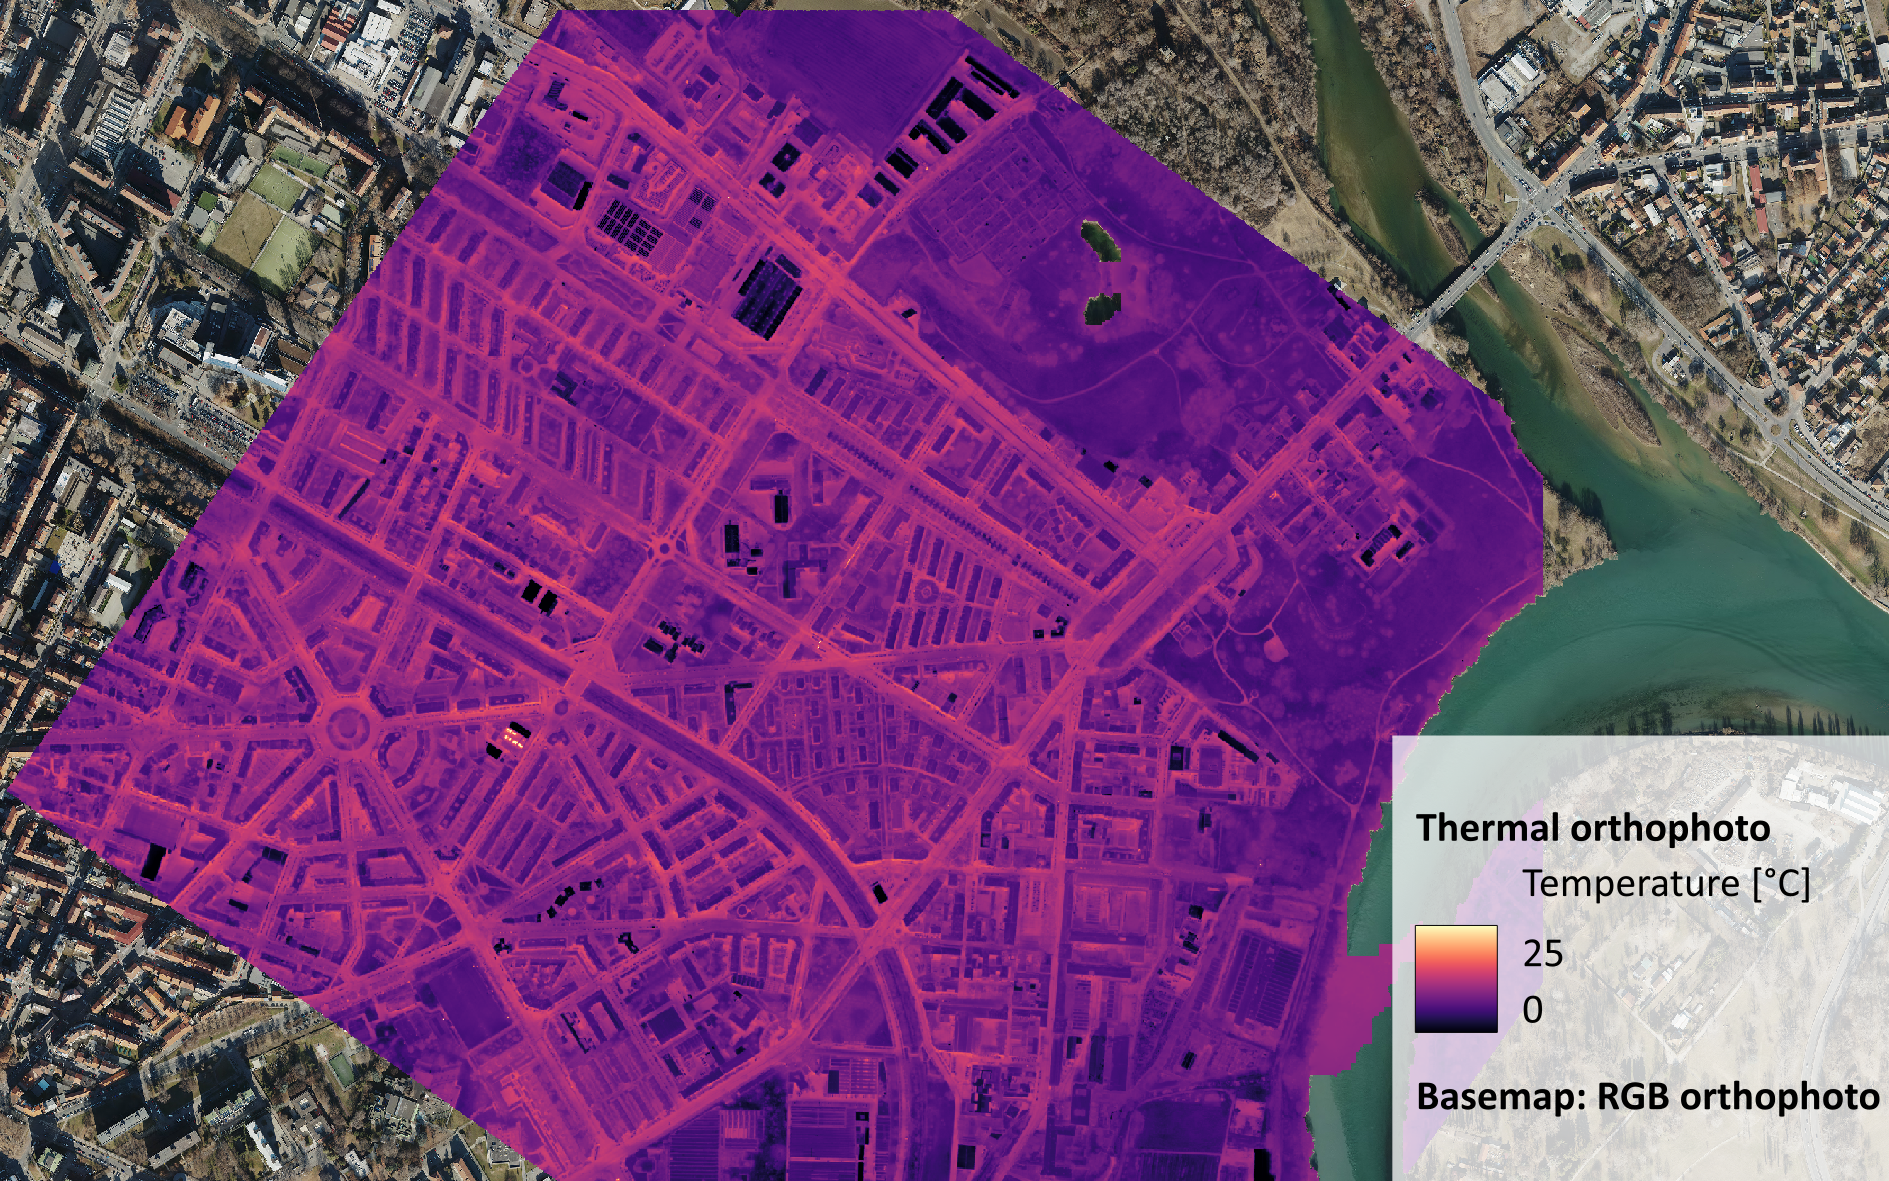
\includegraphics[height=0.6\linewidth]{figs/Thermographic picture_legend.pdf}
    \caption{ Turin Aerial Imagery}
    \label{fig:therm-ortho}
\end{figure}
\begin{figure*}[t]
\centering
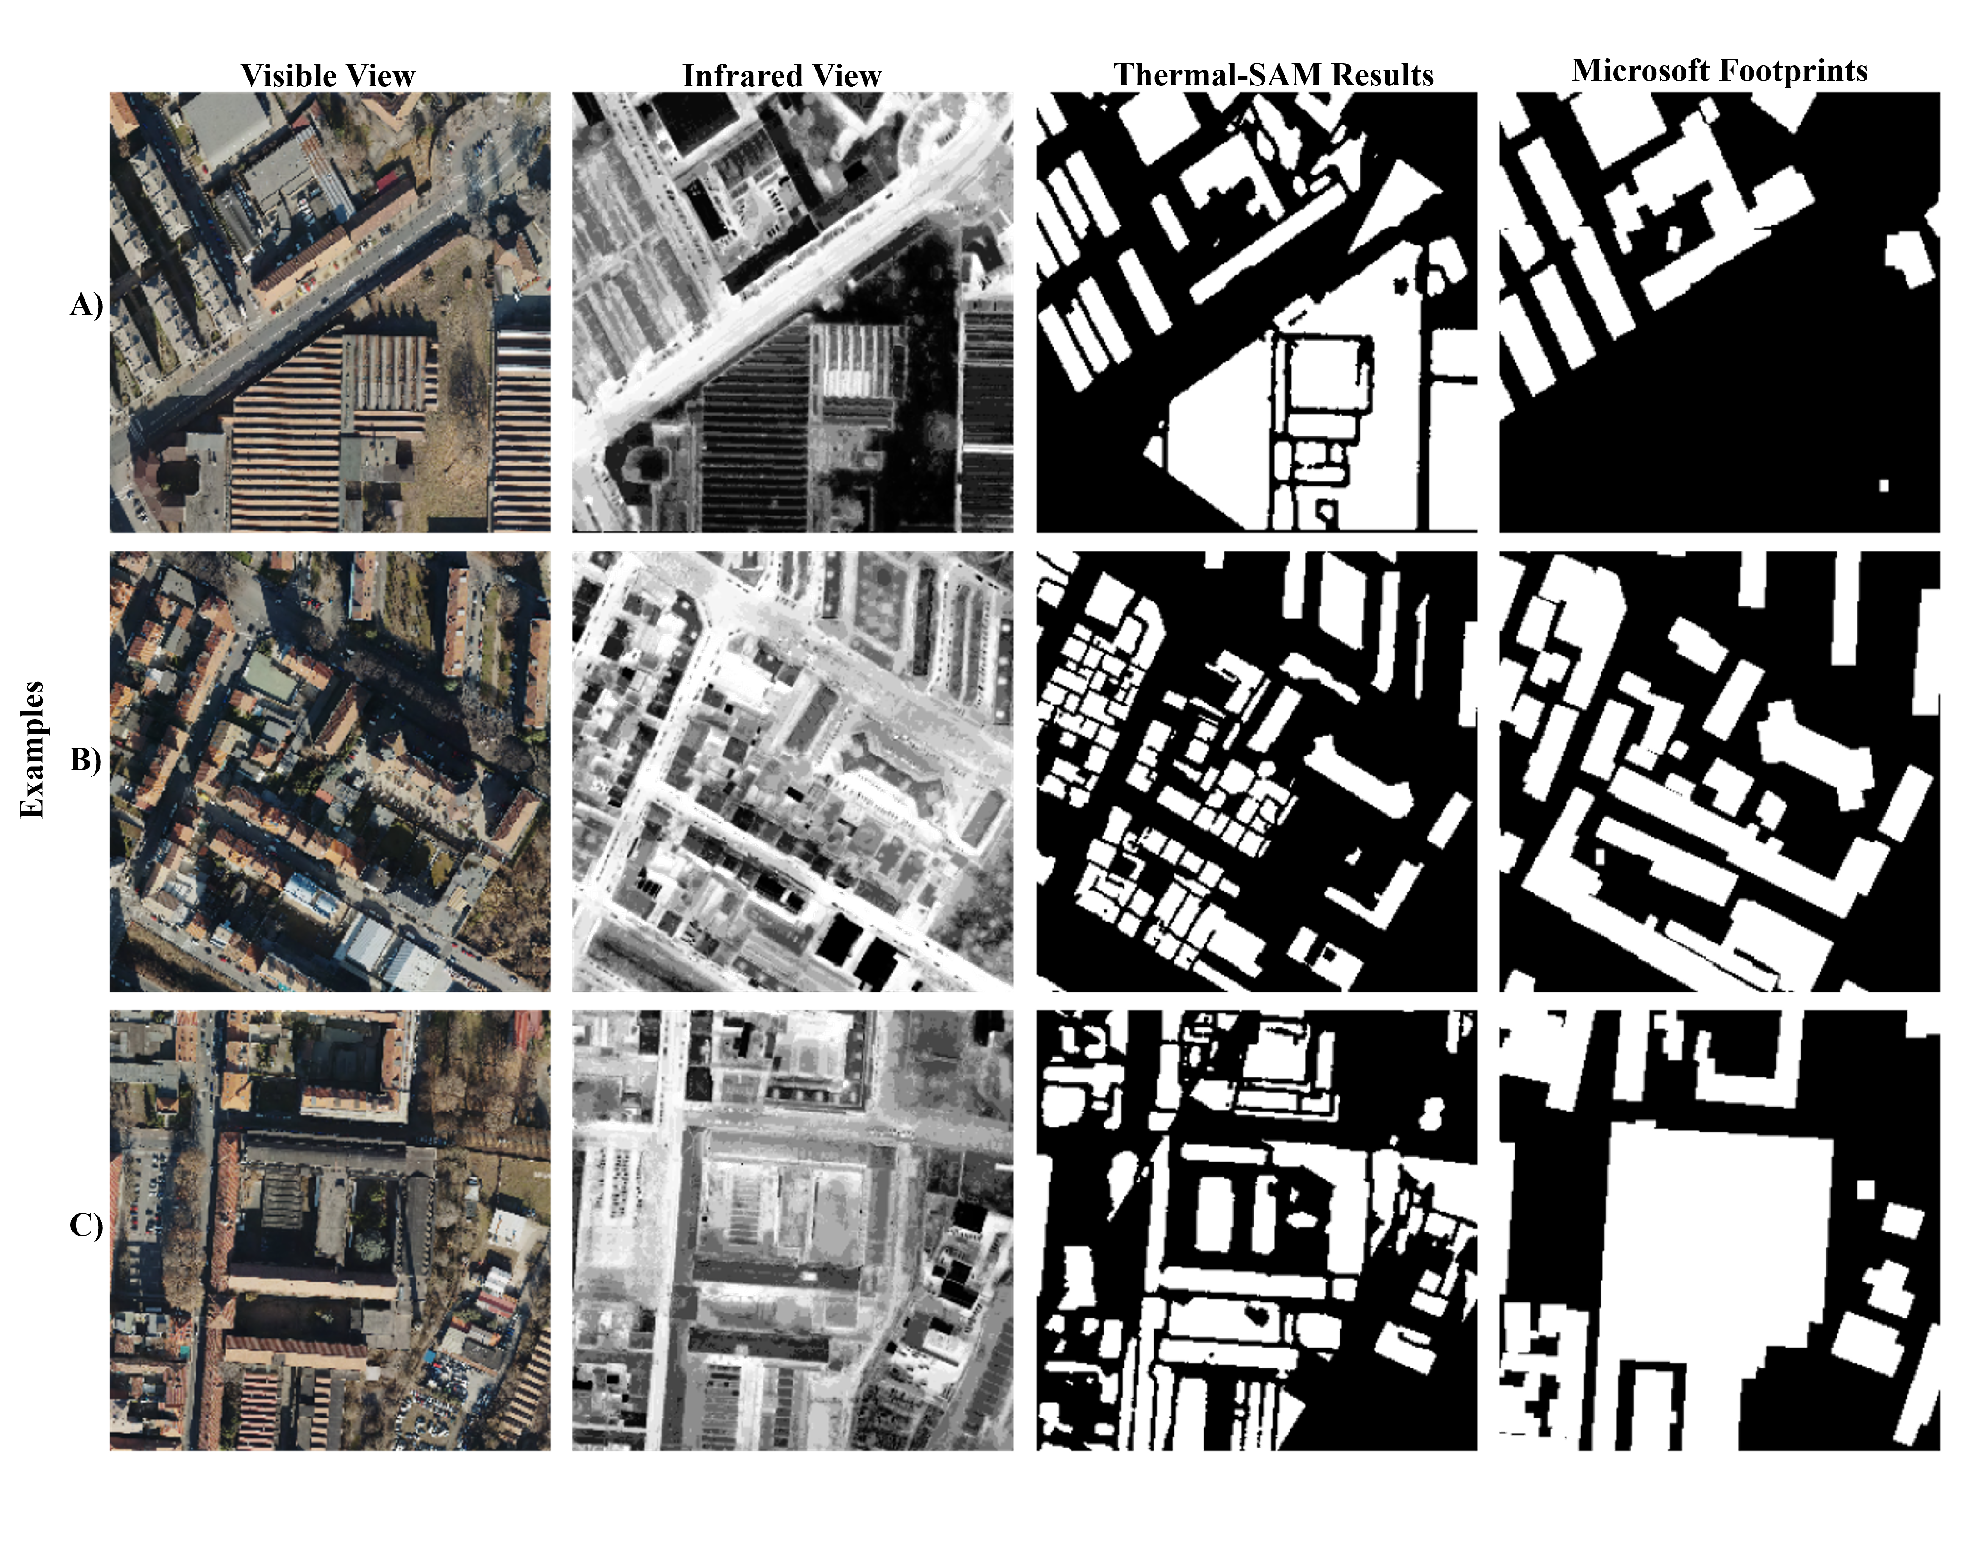
\includegraphics[height=0.71\linewidth]{figs/compre_results_ev.pdf}
\caption{Qualitative Comparison of Building Segmentation: Thermal-SAM vs. Microsoft Footprints}
\label{fig:segresultsms}
\end{figure*}


\subsection{Infrared View and Visible View}
We use a UAV with thermal camera to capture the dataset. During the UAV flight, skies were mostly clear with an ambient temperature around 20$\degree$ C, ensuring stable conditions for midwave infrared capture despite possible variability from clouds or wind. Thermal images were captured by FLIR A8581 MWIR HD camera (equipped in a UAV), shortly after sunset, to minimize biases from solar heating, flying at or above 300m in a nadir orientation as legally mandated.  This altitude was chosen to balance coverage of our 2$km^2$ study region with achieving a fine ground sampling distance (~20cm) for distinguishing building rooftops. We also verified the camera’s $\pm$ 1 $\degree C$ accuracy by referencing a known temperature target on the ground before and after the flight. Midwave IR generally provides a higher spatial resolution than longwave IR, resulting in a ground sampling distance of approximately 20cm—relatively fine for thermal imaging. However, due to the lower photon energy compared to the visible spectrum (0.4–0.7 $\mu m$), a larger instantaneous field of view is required to capture sufficient radiation, which can make thermal images coarser or noisier than their RGB counterparts. Nevertheless, we produced a final orthomosaic of roughly 7,814 $\times$ 6,000 pixels, as shown in Figure~\ref{fig:therm-ortho}. 
Concurrently, color aerial images were captured from the same vantage, offering a higher resolution of 39,070 × 30,000 pixels, as shown by the purple overlay in Figure~\ref{fig:therm-ortho}. Although these RGB images exhibit sharper detail due to their shorter wavelengths, combining them with midwave IR data allows us to capture both temperature patterns and fine-grained scene structure—a key advantage for unsupervised segmentation tasks.

\subsection{Data Preprocessing}
Both the infrared and visible views underwent an orthorectification process to correct for perspective distortions and terrain effects, ensuring that each pixel is accurately aligned with real-world coordinates in WGS84. We used standard aerial triangulation and ground control points to refine the mosaics, then performed a global shift-rotation alignment of the IR mosaic to match the RGB mosaic, ensuring that patches cover the same region. Although this alignment simplifies subsequent patching and segmentation, it cannot entirely eliminate the minor distortions between corresponding buildings in the two views.

\subsection{Microsoft Footprints}
Microsoft  Footprint (MF) \footnote{https://github.com/microsoft/GlobalMLBuildingFootprints} is a global dataset released by Bing Maps that comprises 1.4 billion building footprints extracted from imagery captured between 2014 and 2024. The building labels are generated by deep neural networks (DNNs) trained for semantic segmentation, which detect building pixels in color aerial images and convert these detections into polygonal representations. Although these labels may not be perfectly accurate due to the absence of human annotation, we still use the subset of Footprint data covering Turin, Italy, as the an evaluation indicator for our quantitative evaluation.

\subsection{Implementation Details}
In our experiments, we utilized the PyTorch framework (version 2.0.1) within a CUDA 11.7 environment. We employed the Adam optimizer with an initial learning rate of $1e^{-5}$, and a scheduled learning rate adjustment. The experiments were conducted on high-performance NVIDIA Tesla V100 GPUs. For pseudo-label generation, we used SAM-huge, OneFormer-large, and Clip-Seg-refined. For fine-tuning, we used SAM-base.
\subsection{Qualitative Comparison of MF}

In Section 4.3, although we employed Microsoft Footprints as an evaluation indicator to compute metrics, it is important to note that these footprints do not represent the true mask labels. Therefore, in this section, we present three examples (A, B, and C) to visually compare our results with Microsoft Footprints. The first two columns display the visible and infrared views of three aerial images. 

When comparing the segmentation results generated by our Thermal-SAM model with those of Microsoft Footprints, our approach demonstrates higher precision by detecting more complete building structures and capturing finer details, particularly evident in Example A. In this example, a large area in the lower portion of the visible view is easily misclassified as farmland from visible view; Microsoft Footprints do not include labels for this region, whereas our Thermal-SAM successfully segments the buildings using only the infrared view.

Furthermore, in Examples B and C, Microsoft Footprints assigns a single, large mask to high-density building areas, failing to distinguish individual small buildings. In contrast, our model effectively segments each small building, with Example B being particularly noteworthy. These results underscore our model's effectiveness in achieving accurate building segmentation in thermal imagery.


\end{document}


% This document was modified from the file originally made available by
% Pat Langley and Andrea Danyluk for ICML-2K. This version was created
% by Iain Murray in 2018, and modified by Alexandre Bouchard in
% 2019 and 2021 and by Csaba Szepesvari, Gang Niu and Sivan Sabato in 2022.
% Modified again in 2023 and 2024 by Sivan Sabato and Jonathan Scarlett.
% Previous contributors include Dan Roy, Lise Getoor and Tobias
% Scheffer, which was slightly modified from the 2010 version by
% Thorsten Joachims & Johannes Fuernkranz, slightly modified from the
% 2009 version by Kiri Wagstaff and Sam Roweis's 2008 version, which is
% slightly modified from Prasad Tadepalli's 2007 version which is a
% lightly changed version of the previous year's version by Andrew
% Moore, which was in turn edited from those of Kristian Kersting and
% Codrina Lauth. Alex Smola contributed to the algorithmic style files.
